
%(BEGIN_QUESTION)
% Copyright 2011, Tony R. Kuphaldt, released under the Creative Commons Attribution License (v 1.0)
% This means you may do almost anything with this work of mine, so long as you give me proper credit

Calculate the following values in this balanced three-phase power system, assuming a total power of 9.2 kW:

$$\includegraphics[width=15.5cm]{i02143x01.eps}$$

\begin{itemize}
\item{} $V_{line}$ = \underbar{\hskip 50pt} volts
\vskip 10pt
\item{} $I_{line}$ = \underbar{\hskip 50pt} amps 
\vskip 10pt
\item{} $V_{phase}$ (load) = \underbar{\hskip 50pt} volts 
\vskip 10pt
\item{} $I_{phase}$ (load) = \underbar{\hskip 50pt} amps 
\vskip 10pt
\item{} Power factor = \underbar{\hskip 50pt}
\end{itemize}

\underbar{file i02143}
%(END_QUESTION)





%(BEGIN_ANSWER)

\begin{itemize}
\item{} $V_{line}$ = \underbar{\bf 1334} volts
\vskip 10pt
\item{} $I_{line}$ = \underbar{\bf 3.983} amps 
\vskip 10pt
\item{} $V_{phase}$ (load) = \underbar{\bf 1334} volts 
\vskip 10pt
\item{} $I_{phase}$ (load) = \underbar{\bf 2.299} amps 
\vskip 10pt
\item{} Power factor = \underbar{\bf 1}
\end{itemize}


%(END_ANSWER)





%(BEGIN_NOTES)

{\bf This question is intended for exams only and not worksheets!}.

%(END_NOTES)

